\chapter{Results and Discussion}
\label{ch:results}

This chapter reports the designs \ac{SA} found in every case study (Section~\ref{sec:res-cases}),
shows them at work (Section~\ref{sec:res-vis}), analyses what the optimiser learned
(Section~\ref{sec:res-learned}) and then analyses the algorithm itself: convergence, cost and
repeatability (Section~\ref{sec:res-perf}) and the effect of its parameters
(Section~\ref{sec:params}).

\section{Fleets designed for every case study}
\label{sec:res-cases}
Table~\ref{tab:caseresults} lists the results of all \ac{SA} runs. Every final design is
feasible.

\begin{table}[htbp]
\centering
\caption{Fleets designed by \ac{SA} in every case study (mean over runs; $N$ is listed per run)}
\label{tab:caseresults}
\scriptsize
\begin{tabular}{@{}lllcllcccccc@{}}
\toprule
Case & Body & $T_{\max}$ & $N_{\max}$ & $N$ per run & $T$ & $J$ (mean $\pm$ std) & $C$ & $Z$ & $E$ & $T/T_{\max}$ & Feas. \\
\midrule
A1 & Eros & 10 d & 5 & 3, 2, 2, 2, 2 & 2.03 d & 0.108 $\pm$ 0.006 & 95.1\,\% & 0.22 & 0.066 & 0.20 & 5/5 \\
A2 & Eros & 1 d & 5 & 3, 2, 3, 3, 4 & 10.9 h & 0.212 $\pm$ 0.012 & 88.6\,\% & 0.30 & 0.129 & 0.45 & 5/5 \\
A3 & Eros & 1 d & 10 & 3, 4, 4, 3, 2 & 10.3 h & 0.205 $\pm$ 0.013 & 89.6\,\% & 0.32 & 0.128 & 0.43 & 5/5 \\
A4 & Eros & 12 h & 10 & 4, 4, 3, 2, 4 & 6.3 h & 0.277 $\pm$ 0.016 & 80.5\,\% & 0.34 & 0.157 & 0.52 & 5/5 \\
A5 & Eros & 6 h & 10 & 3, 4, 2, 3, 5 & 4.5 h & 0.355 $\pm$ 0.024 & 75.0\,\% & 0.34 & 0.192 & 0.75 & 5/5 \\
A6 & Eros & 2 h & 10 & 2, 4, 4, 1, 3 & 0.8 h & 0.443 $\pm$ 0.032 & 38.7\,\% & 0.28 & 0.120 & 0.38 & 5/5 \\
\midrule
B1 & Kleopatra & 3 d & 5 & 3, 3, 3, 2, 2 & 16.6 h & 0.225 $\pm$ 0.012 & 74.8\,\% & 0.26 & 0.091 & 0.23 & 5/5 \\
B2 & Kleopatra & 3 d & 10 & 3, 3, 3, 3, 2 & 20.7 h & 0.231 $\pm$ 0.014 & 76.3\,\% & 0.28 & 0.090 & 0.29 & 5/5 \\
B3 & Kleopatra & 12 h & 10 & 2, 3, 3, 3, 3 & 5.2 h & 0.340 $\pm$ 0.016 & 61.6\,\% & 0.28 & 0.127 & 0.44 & 5/5 \\
\midrule
D & Eros & 10 d & 5 & 2, 2, 2, 2, 2 & 1.16 d & 0.073 $\pm$ 0.004 & 97.9\,\% & 0.20 & 0.063 & 0.12 & 5/5 \\
\bottomrule
\end{tabular}
\end{table}


\textbf{Less time, more spacecraft, and only the time that pays.} Figure~\ref{fig:fleettime} shows
how the designs change with the longest allowed mission on Eros. With ten days available, \ac{SA}
sends two spacecraft (four runs of five) and \emph{ends the mission after about two days} (44--55\,h),
by which time they have imaged 95\,\% of the sunlit area: the asteroid turns about nine times under
every orbit in two days, after which the coverage gained per extra day is worth less than its cost
in time ($w_T$). When less time is available the surface no longer comes to the spacecraft, so more
spacecraft are sent: two to four at one day and twelve hours, two to five at six hours, and the
mission uses a larger share of the time allowed (20\,\% of $T_{\max}$ for ten days, 45\,\% for one
day, 75\,\% for six hours). Coverage falls from 95\,\% (ten days) to 89\,\% (one day), 81\,\% (twelve
hours) and 75\,\% (six hours). At two hours Eros turns by only a third of a revolution and each
spacecraft takes at most a dozen frames, so coverage collapses to 39\,\% and the runs disagree (1 to 4
spacecraft); here \ac{SA} even stops after 0.5--1\,h, because the last frames add too little.
\ac{SA} never fills all the slots it is allowed: with $N_{\max}=10$ it sends the same 2--4 spacecraft
as with $N_{\max}=5$, because each spacecraft has to pay for itself through coverage.

\begin{figure}[htbp]
\centering
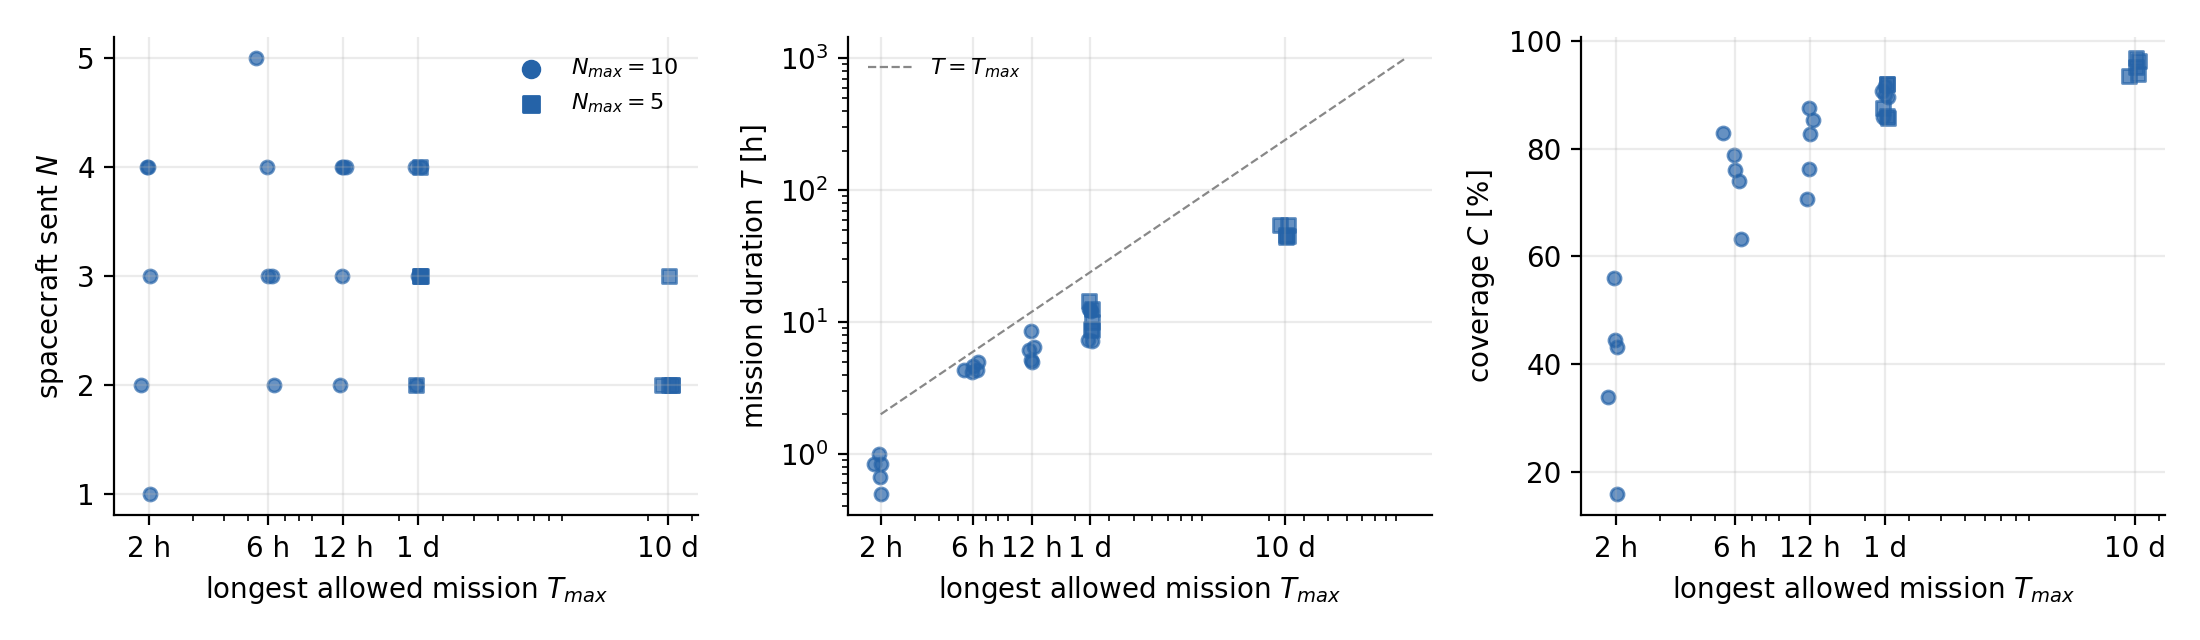
\includegraphics[width=\textwidth]{Figures/fig_fleet_vs_time.png}
\caption{Eros: fleet size, mission duration and coverage chosen by \ac{SA} against the longest
allowed mission $T_{\max}$ (each marker is one run).}
\label{fig:fleettime}
\end{figure}

\textbf{Second body.} The same code and settings, applied to Kleopatra (46 times the surface of Eros),
send two or three spacecraft for 12--33\,h when three days are allowed and image 75--76\,\% of the
sunlit area; with twelve hours they send two or three spacecraft for about five hours and image
62\,\%. Coverage is lower than for Eros with a comparable mission length because Kleopatra is much
more concave (it fills only 64\,\% of its convex hull against 84\,\% for Eros): the narrow waist between
its two lobes hides part of the surface from most viewing directions (Figure~\ref{fig:progB1}).

\section{The best designs at work}
\label{sec:res-vis}
Figures~\ref{fig:progA1}--\ref{fig:progB1} replay the best designs of three cases in the viewer
(on the 6\,000-facet Eros model for display; green: photographed so far, grey: not yet,
blue: never sunlit during the mission).

\begin{figure}[htbp]
\centering
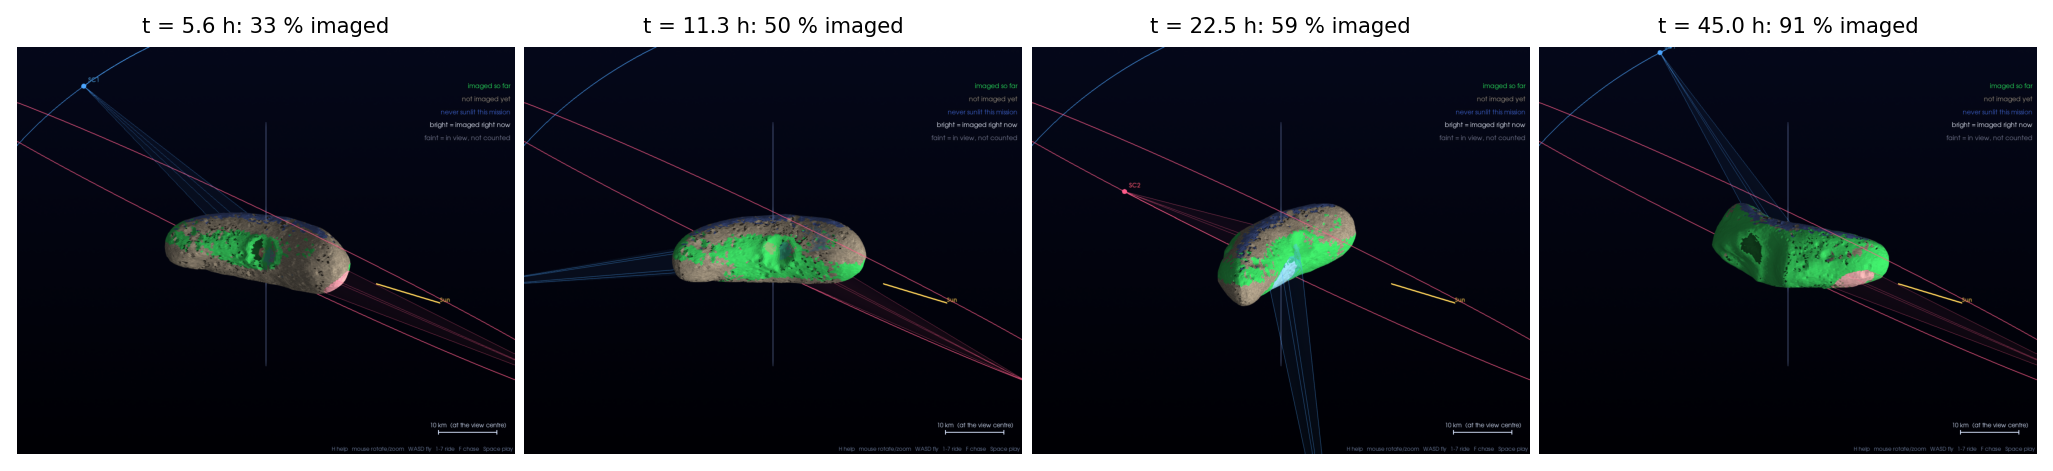
\includegraphics[width=\textwidth]{Figures/progress_A1.png}
\caption{Case A1 (Eros, $T_{\max}=10$\,d): the best design at four moments of its mission.}
\label{fig:progA1}
\end{figure}

\begin{figure}[htbp]
\centering
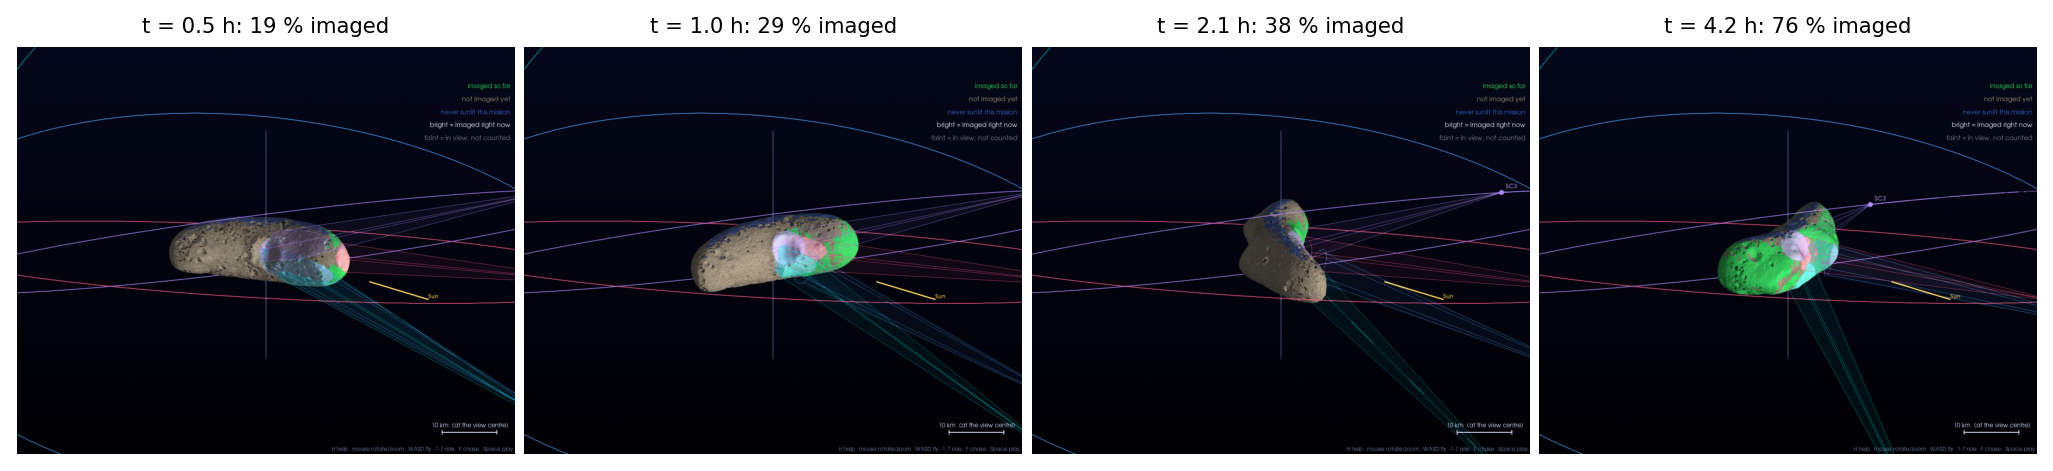
\includegraphics[width=\textwidth]{Figures/progress_A5.png}
\caption{Case A5 (Eros, $T_{\max}=6$\,h): the best design at four moments of its mission.}
\label{fig:progA5}
\end{figure}

\begin{figure}[htbp]
\centering
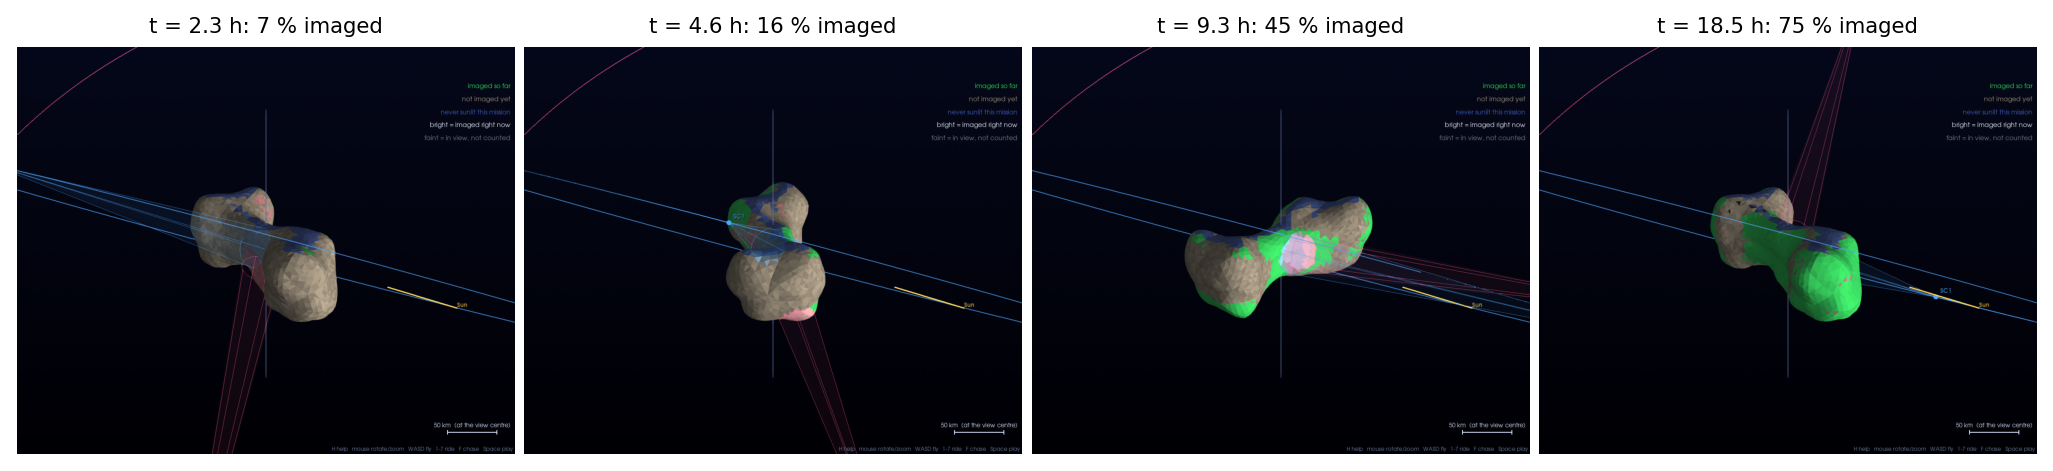
\includegraphics[width=\textwidth]{Figures/progress_B1.png}
\caption{Case B1 (Kleopatra, $T_{\max}=3$\,d): the best design at four moments of its mission.}
\label{fig:progB1}
\end{figure}

The replays show how the fleets work. In the ten-day case (Figure~\ref{fig:progA1}) the two
spacecraft see about a third of the sunlit area in the first rotation of Eros; the rest is collected
as the spin brings new longitudes under the orbits, and the mission is stopped once the remaining
facets come in too slowly to pay for more time. In the six-hour case
(Figure~\ref{fig:progA5}) four spacecraft are spread around the body in different planes so that,
together, they see both ends of Eros within about one rotation. On Kleopatra
(Figure~\ref{fig:progB1}) two spacecraft image three quarters of the sunlit area in 18.5\,h. The coverage
values in the figure titles are computed on the 6\,000-facet display model, so they are a few
points lower than those of Table~\ref{tab:caseresults} (validation V7).

\section{What the optimiser learned}
\label{sec:res-learned}

\begin{figure}[htbp]
\centering
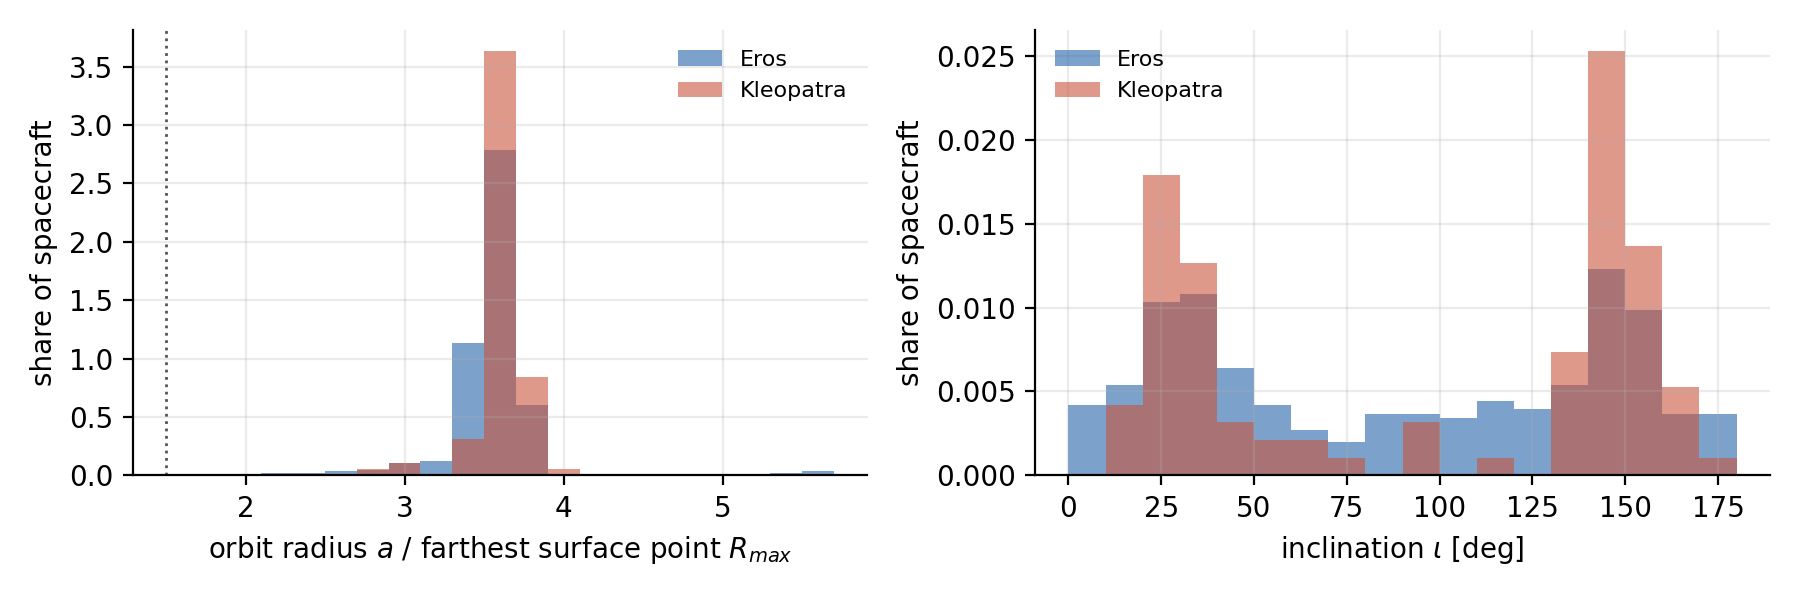
\includegraphics[width=0.9\textwidth]{Figures/fig_orbits.png}
\caption{Orbits of every spacecraft in the best feasible \ac{SA} designs: radius in units of the
farthest surface point (dotted line: $r_{\min}=1.5R_{\max}$) and inclination.}
\label{fig:orbits}
\end{figure}

Figure~\ref{fig:orbits} collects every orbit of the best designs and reveals two consistent rules.
\begin{itemize}
\item \textbf{The same height in proportion to the body.} The orbit radii cluster tightly at
3.5--3.6 times the farthest surface point for \emph{both} bodies (median 62.4\,km for Eros, 409\,km
for Kleopatra; 79\,\% and 88\,\% of the orbits lie within $\pm$5\,\% of the median). This is just above the usable
camera range (58.6\,km and 391\,km): the optimiser flies as high as it can while the near side of the
body is still within range, which maximises the footprint of every frame. Nothing in the code tells
it this; it emerges from the simulation, and it scales correctly from a 34\,km to a 219\,km body.
\item \textbf{Tilted, not polar, orbits.} The median tilt of the orbits from the equator is
35$^\circ$ for Eros and 31$^\circ$ for Kleopatra. With the Sun in the equatorial plane, facets near
the poles never see the Sun 20$^\circ$ above their horizon and are not part of $A^{*}$, so a polar
orbit would spend time over regions that do not count; a moderate tilt, combined with the spin and
the 65$^\circ$ emission limit, sweeps the whole lit band. Prograde and retrograde orbits are about
equally common (50\,\% and 57\,\% retrograde): the extra plane-change $\Delta V$ of a retrograde orbit
changes $J$ by only about 0.003, so the fitness hardly distinguishes them.
\item \textbf{Batteries are never the limit; separation sometimes is.} Re-evaluating the 45 best
designs of cases A and B, the lowest battery charge is 58\,\% (limit 20\,\%) and the median is
100\,\%: the 180\,W panels more than cover the 50\,W bus plus imaging.
Separation, in contrast, is close to active in three short-mission Eros designs (closest approach
2.7--3.0\,km against the 2\,km limit), where several spacecraft share the space just above the camera
range.
\end{itemize}

\section{Algorithm performance}
\label{sec:res-perf}

\begin{figure}[htbp]
\centering
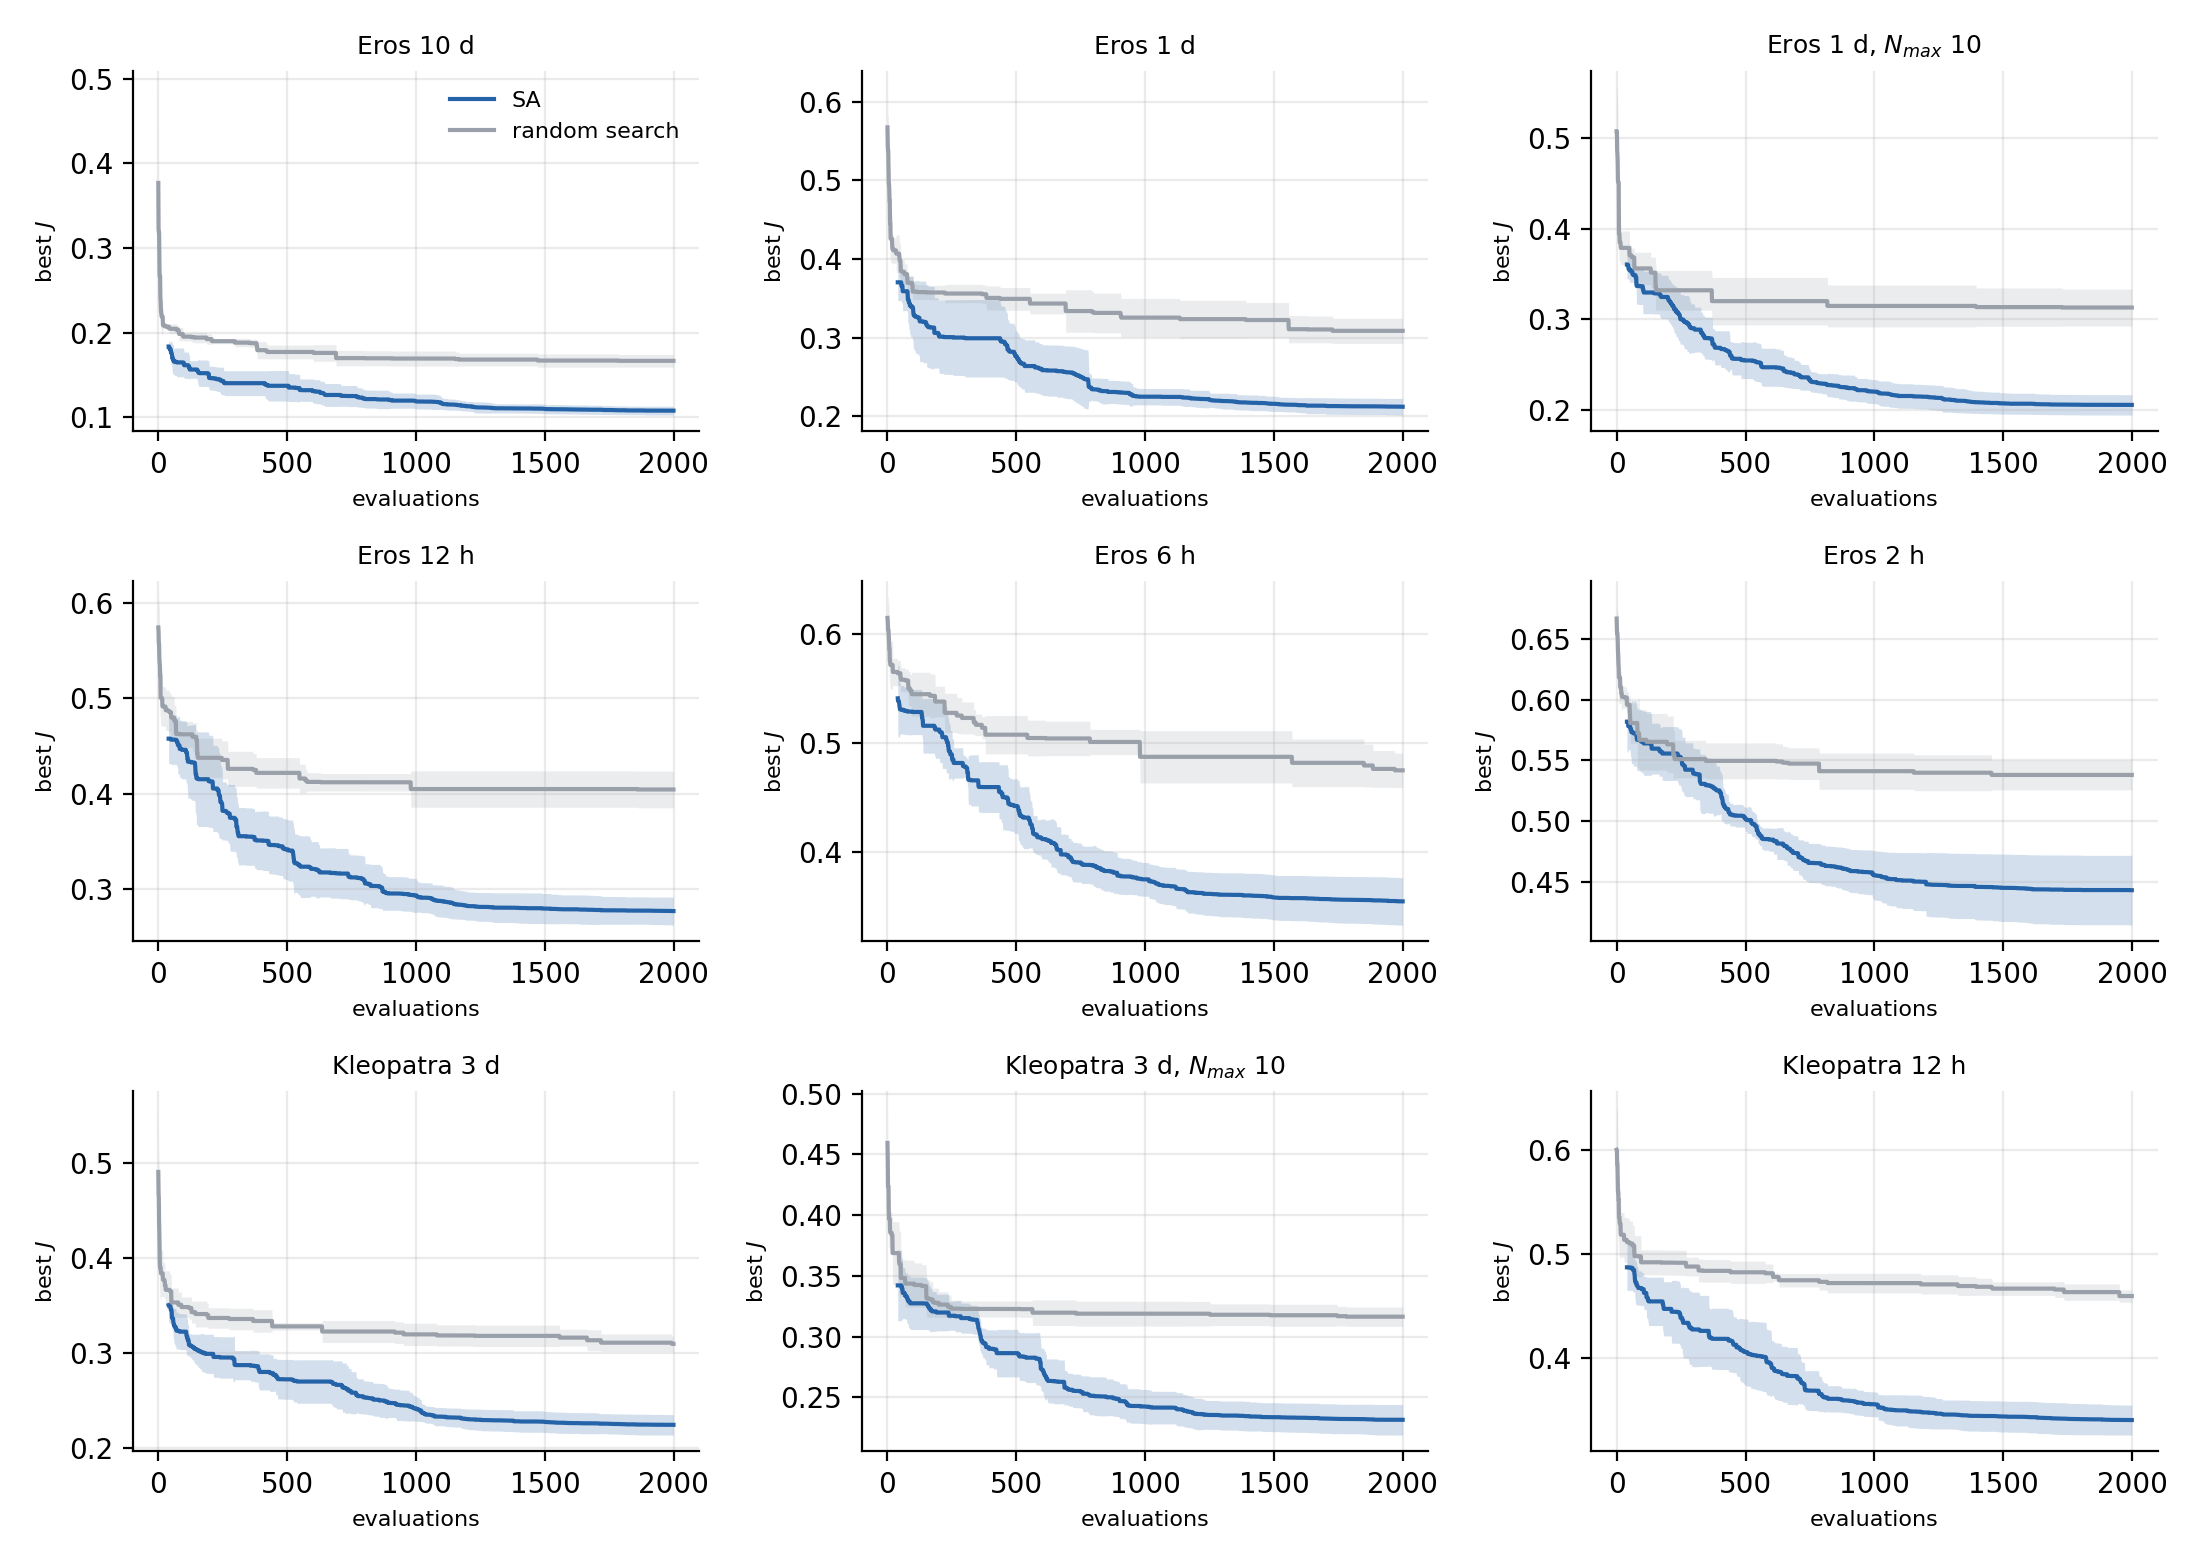
\includegraphics[width=\textwidth]{Figures/fig_convergence.png}
\caption{Convergence: best fitness against evaluations, mean $\pm$ one standard deviation over 5
runs, for \ac{SA} and random search in every case of A and B.}
\label{fig:conv}
\end{figure}

\textbf{Convergence.} Figure~\ref{fig:conv} shows that \ac{SA} improves quickly during the first
500--1000 evaluations, while the temperature is high and large moves are accepted, and then
fine-tunes the orbits; by 1500 evaluations the curves are nearly flat, so the budget of 2000 is
adequate. Random search improves only in rare jumps and stalls early, because the chance of drawing a
better design at random falls quickly. The warm start is visible as \ac{SA}'s curves starting at
evaluation 40, already at a level random search reaches only after a hundred or more draws.

\textbf{Repeatability.} The standard deviation of the final $J$ over five seeds is 0.006--0.016 in
most cases and 0.024--0.032 for the hardest, six- and two-hour Eros missions
(Table~\ref{tab:caseresults}). Different seeds therefore give designs of very similar quality, but
not identical designs: the fleet size in particular differs between runs where the fitness is flat in
$N$ (validation V6).

\textbf{Computational cost.} Table~\ref{tab:cost} gives the time of one run on one CPU core. It grows
with the number of time steps and facets, from a few seconds for a two-hour Eros mission to about
3--4 minutes for ten days on Eros or three days on Kleopatra. It hardly depends on $N_{\max}$, because
a move changes at most two spacecraft and the unchanged ones are taken from the track cache. The same
cache explains why random search, which simulates every spacecraft of every new design from scratch,
is up to five times slower than \ac{SA} for the same number of evaluations (e.g.\ 7.1 against 2.9 minutes for
ten days on Eros). The whole validation (193 runs) took about one hour on six cores.

\section{Effect of the algorithm parameters}
\label{sec:params}
Case~E changes one parameter at a time from the defaults (Table~\ref{tab:saparams}) on the
two-day Eros mission ($N_{\max}=5$), with five runs per setting: the cooling factor $\alpha$
(fixed at 0.80, 0.95 or 0.98 instead of fitted to the budget, in which case a run stops when
$\Theta<10^{-3}\Theta_0$ even if budget is left), the initial acceptance probability $p_0$
(0.3, 0.8, 0.95), the initial step $\sigma_0$ (0.05, 0.10, 0.50) and the warm start (one random
start instead of the best of 20).

\begin{table}[htbp]
\centering
\caption{Case E: effect of the \ac{SA} parameters (Eros, $T_{\max}=2$\,d, $N_{\max}=5$; one parameter changed at a time from the defaults)}
\label{tab:sa-params}
\scriptsize
\begin{tabular}{@{}lcccccccc@{}}
\toprule
Setting & $\alpha$ used & Runs & $J$ (mean $\pm$ std) & Best & Worst & Mean $C$ & Mean $N$ & Evaluations \\
\midrule
default & 0.912 & 5 & 0.1602 $\pm$ 0.0044 & 0.1540 & 0.1645 & 92.3\,\% & 2.4 & 2000 \\
$\alpha=$ 0.80 & 0.800 & 5 & 0.1930 $\pm$ 0.0267 & 0.1591 & 0.2273 & 92.2\,\% & 2.6 & 846 \\
$\alpha=$ 0.95 & 0.950 & 5 & 0.1674 $\pm$ 0.0027 & 0.1635 & 0.1702 & 90.3\,\% & 2.4 & 2000 \\
$\alpha=$ 0.98 & 0.980 & 5 & 0.2082 $\pm$ 0.0155 & 0.1889 & 0.2225 & 85.6\,\% & 2.8 & 2000 \\
$p_0=$ 0.30 & 0.912 & 5 & 0.1626 $\pm$ 0.0110 & 0.1503 & 0.1781 & 91.2\,\% & 2.6 & 2000 \\
$p_0=$ 0.80 & 0.912 & 5 & 0.1720 $\pm$ 0.0136 & 0.1635 & 0.1956 & 89.9\,\% & 2.6 & 2000 \\
$p_0=$ 0.95 & 0.912 & 5 & 0.2065 $\pm$ 0.0275 & 0.1824 & 0.2508 & 87.6\,\% & 2.6 & 2000 \\
$\sigma_0=$ 0.05 & 0.912 & 5 & 0.1883 $\pm$ 0.0219 & 0.1607 & 0.2215 & 88.2\,\% & 2.4 & 2000 \\
$\sigma_0=$ 0.10 & 0.912 & 5 & 0.1887 $\pm$ 0.0407 & 0.1552 & 0.2538 & 88.7\,\% & 2.2 & 2000 \\
$\sigma_0=$ 0.50 & 0.912 & 5 & 0.1600 $\pm$ 0.0074 & 0.1521 & 0.1714 & 92.3\,\% & 2.8 & 2000 \\
one random start & 0.913 & 5 & 0.1593 $\pm$ 0.0055 & 0.1532 & 0.1674 & 92.0\,\% & 2.4 & 2000 \\
\bottomrule
\end{tabular}
\end{table}


\begin{figure}[htbp]
\centering
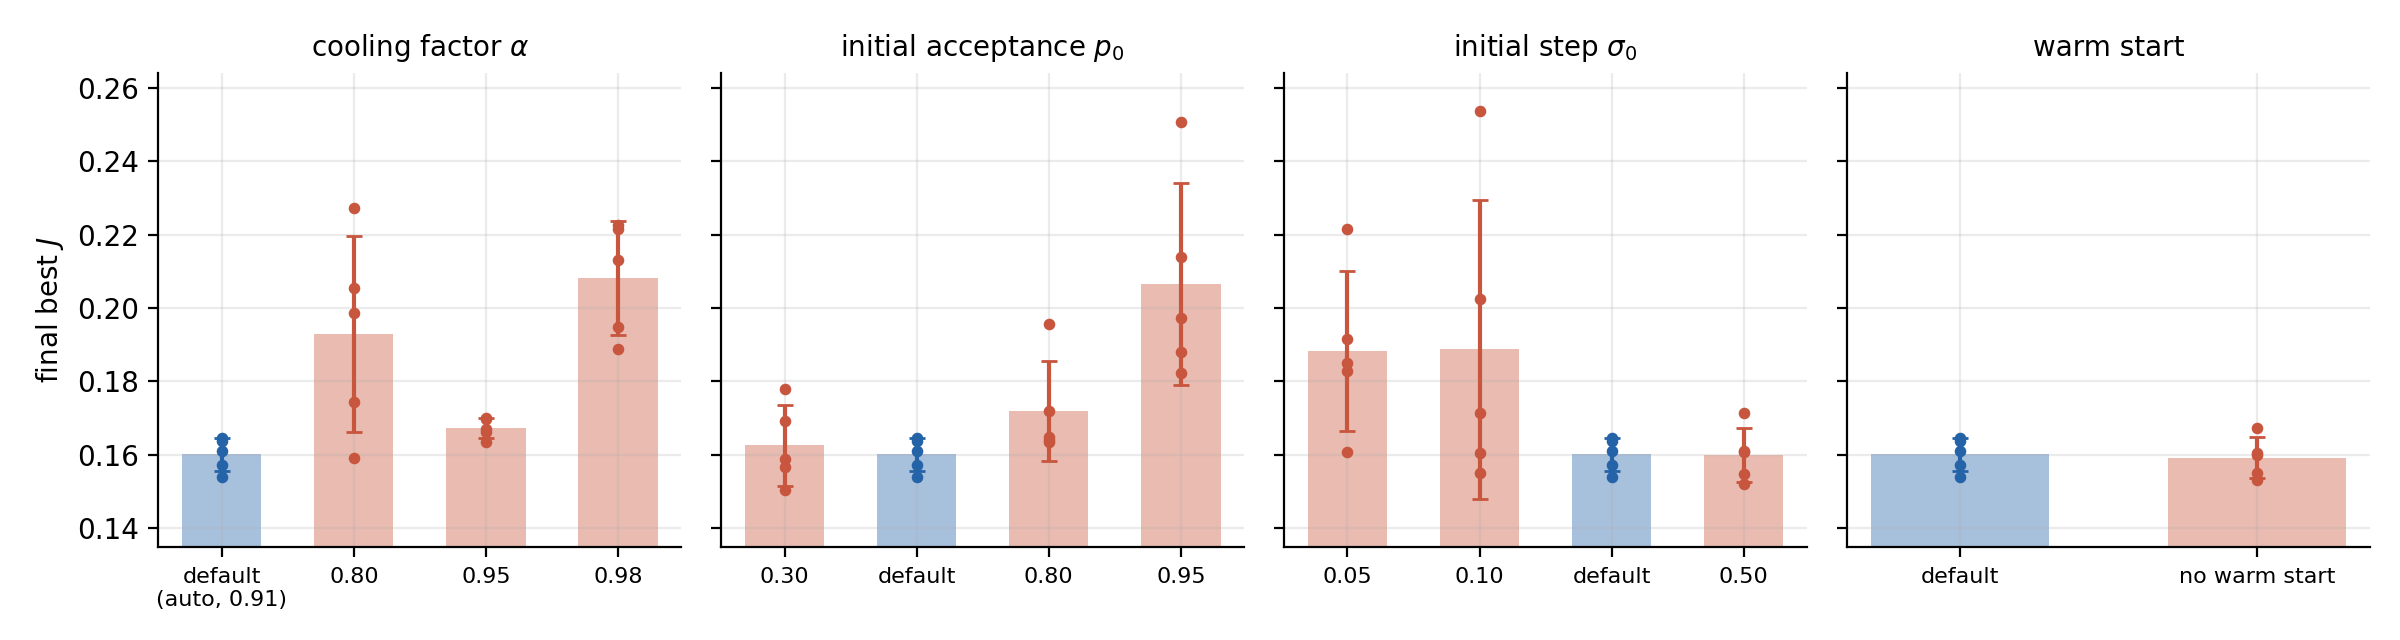
\includegraphics[width=\textwidth]{Figures/fig_params.png}
\caption{Case E: final best fitness for each parameter value (bars: means, dots: runs; blue: the
default).}
\label{fig:params}
\end{figure}

\begin{figure}[htbp]
\centering
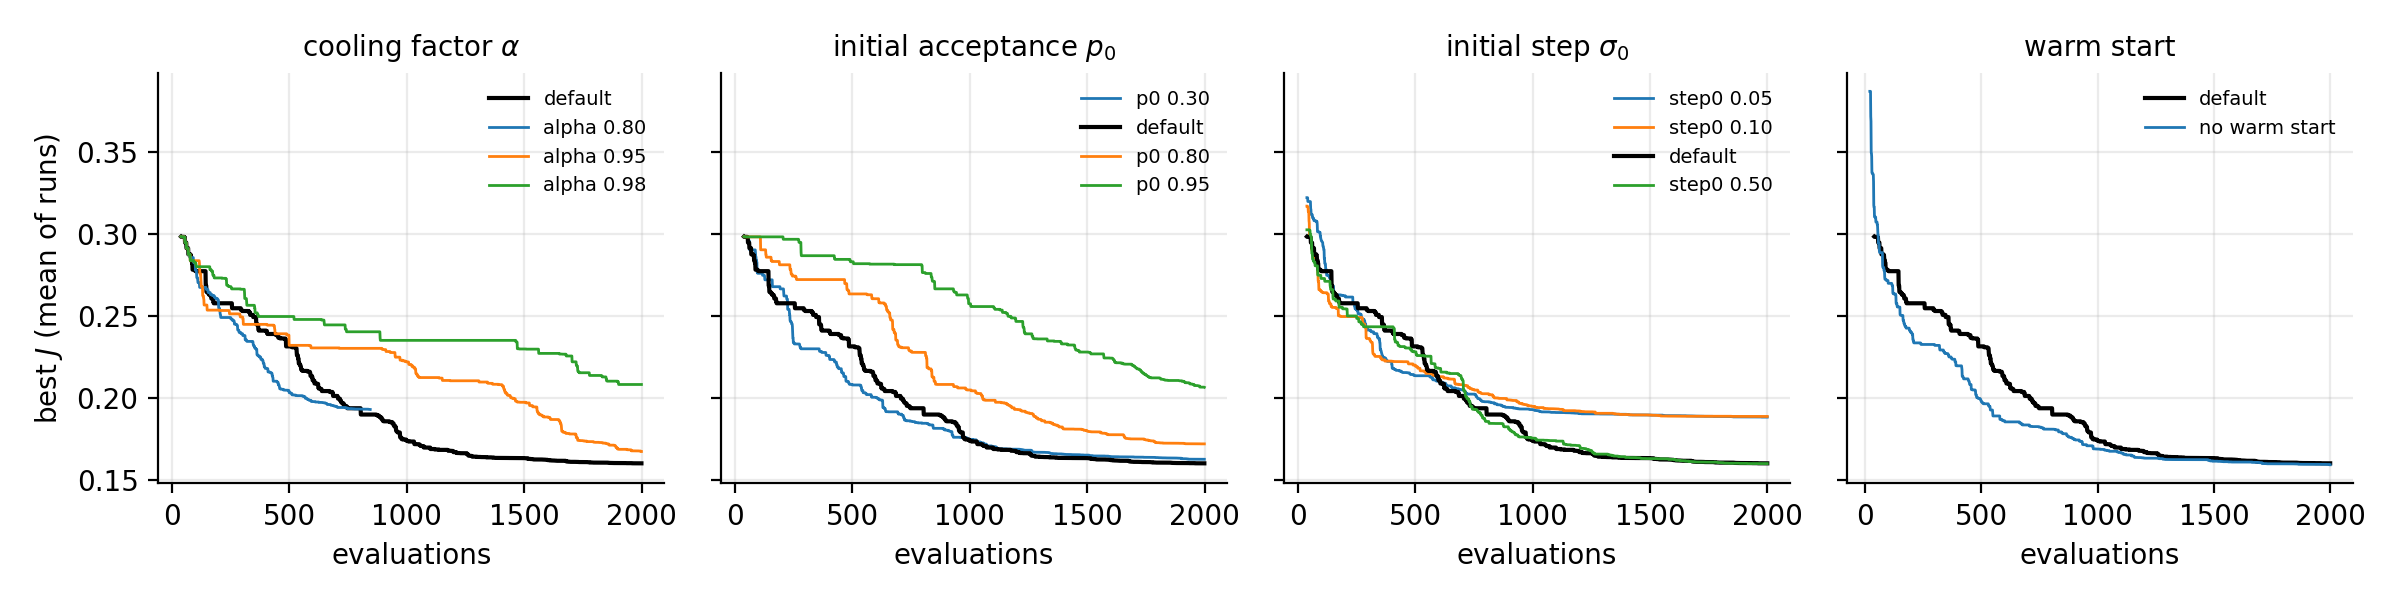
\includegraphics[width=\textwidth]{Figures/fig_params_convergence.png}
\caption{Case E: mean convergence for each parameter value.}
\label{fig:paramsconv}
\end{figure}

\textbf{Cooling factor $\alpha$: the most important parameter.} The default, $\alpha$ fitted to the
budget (0.912 here), gives the best and most consistent result ($J=0.160\pm0.004$). A fixed
$\alpha=0.80$ cools so fast that the temperature reaches $10^{-3}\Theta_0$ after only 846 evaluations:
the run ends early, frozen in whatever region it reached, and the results scatter widely
($0.193\pm0.027$). The slow schedules waste the budget on the opposite side: with $\alpha=0.95$ the
temperature at the end of the budget is still 2\,\% of $\Theta_0$ and with $\alpha=0.98$ still 22\,\%,
so the search never settles to fine-tune ($J=0.167$ and $0.208$). Fitting $\alpha$ to the budget
avoids both failures automatically.

\textbf{Initial acceptance $p_0$: do not start too hot.} $p_0=0.3$ and $0.5$ give the same quality;
$p_0=0.8$ and especially $0.95$ are clearly worse ($0.172$ and $0.207$). A hot start accepts almost
every worsening move for the first part of the run (the flat green and orange curves of
Figure~\ref{fig:paramsconv}), so a large part of the budget is spent on a random walk.

\textbf{Initial step $\sigma_0$: start with large moves.} $\sigma_0=0.25$ (default) and $0.5$ are
equally good ($0.160$), while small initial steps ($0.05$, $0.10$) are worse and much less reliable
($0.188\pm0.022$ and $0.189\pm0.041$): with small steps \ac{SA} cannot move an orbit far enough to
leave a poor region, so the outcome depends on where it started.

\textbf{Warm start: no effect here.} Starting from one random design instead of the best of 20 gives
the same result ($0.159$ against $0.160$) in this case. The 20 start evaluations are a small part of the
budget, and the adaptive $\Theta_0$ and the cooling recover from a poor start when the mission is two
days long and most orbits see something. The warm start was introduced for the flat regions of short
missions and high orbits; in this case it is neutral and costs only 1\,\% of the budget.

With five runs per setting the differences above about 0.01 in mean $J$ are consistent with the spread
of the runs; smaller differences (for instance between $p_0=0.3$ and $0.5$, or $\sigma_0=0.25$ and
$0.5$) should be read as ties.

\section{Recommendations}
\begin{itemize}
\item \textbf{Let the cooling follow the budget.} Fit $\alpha$ so that the temperature reaches its final
value when the budget is used; a fixed $\alpha$ is either too fast (the run stops early) or too slow
(it never fine-tunes).
\item \textbf{Start moderately warm and with large steps}: $p_0\approx0.3$--$0.5$ and
$\sigma_0\approx0.25$--$0.5$ of each variable's range.
\item \textbf{Budget.} About 1500--2000 evaluations are enough for the problem sizes studied; most of
the gain comes in the first 1000.
\item \textbf{Fleet size.} The fitness is flat in $N$ near the optimum and \ac{SA} tends to send one or two
spacecraft too few; for a final design, run \ac{SA} with the fleet size forced to the chosen $N$ and
its neighbours (as in V6), or use a population-based method that keeps several fleet sizes alive.
\item \textbf{Final numbers.} Re-evaluate the chosen designs on the fine shape model, which lowers the
coverage by about two points.
\end{itemize}
